% Discrete Mathematics Lecture Notes 2013-10-18

\subsection{Hamiltonian Graphs}
\lecturedate[\baselineskip]{2013-10-18}

\begin{definition}
In a \dt{Hamiltonian cycle}, each vertex is visited exactly once (except start/end).
$\text{$G$ is \dt{Hamiltonian}} \iff \exists\;\text{Hamiltonian cycle}.$
\end{definition}

Finding a Hamiltonian cycle in a graph is an NP-complete problem.

\begin{definition}
Let $G=(V,E)$ be a graph.
\[
%\forall v,w\in V :  \rightarrow\text{add $vw$ to $E$}\leadsto \tilde E
\tilde E = E\cup \{vw \mid v,w\in V,\; d(v)+d(w) ≥ |V|\}
\]
Then $[G] = (V,\tilde E)$ is called the \dt{closure} of $G$.
\end{definition}

\Theorem.  $G\text{ Hamiltonian} \iff [G]\text{ Hamiltonian}.$

\ProofForward.
Trivial.

\ProofBackward.
Choose
\begin{gather*}
  v,w\in V: vw \not\in E(G),\;d(v)+d(w) ≥ |V| \\
  H=(V,E\cup \{vw\})
\end{gather*}
Assume $H$ is Hamiltonian and $G$ is not.
This means that $\exists\;\text{Hamiltonian cycle in $H$}$ and it must contain $vw$.
In $H$ containing $vw$, say
\[ v=x_1,x_2,x_3,\ldots,x_n=w,x_1 \qquad(n=|V|)\]
Let
\begin{align*}
    X &=\{x_i \mid x_{i-1}\in \Gamma_G(w), 3 ≤ i ≤ n-1 \}\quad\text{and} \\
    Y &=\{x_i \mid x_i\in \Gamma_G(v), 3 ≤ i ≤ n-1 \}.
\end{align*}

\path{v, x_2, x_3, \ldots, x_{n-1}, w} is a path in $G$.

$v \not\in \Gamma_G(w) \implies |X| = d_G(w) - 1$
because exactly one neighbour is excluded, all the others are counted. $x_1= v$ is not a neighbour by our assumption.

$x_2, x_3, \ldots x_{n-2}$ there is one neighbour $x_{n-1}$ of $w$ which is not counted.

Analogously,
$|Y| = d_G(v) - 1$.

Thus $|X| + |Y| \geq n-2$.

Therefore, $\exists\,i: 3 ≤ i ≤ n-1$ such that
$x_{i-1}\in \Gamma_G(w), x_i\in\Gamma_G(v)$, because we iterate over $n-3$ values.

$\implies \path{v=x_1, x_i, x_{i+1}, \ldots, x_{n-1}, w=x_n, x_{i-1}, x_{i-2}, \ldots, x_2, v=x_1}$

But this is a Hamiltonian cycle in $G$ (contradiction).

If $H$ is not Hamiltonian, you could add other edges, but by the same argument, this will not lead to a Hamiltonian graph.

\textbf{Corollary 1.}
Let $G=(V,E), |V| ≥ 3$, such that
\[
    \forall v,w\in V: vw\not\in E\implies d(v) + d(w) \geq |V|.
\]
Then $G$ is Hamiltonian.

\textbf{Corollary 2.}
If
$\forall v \in V : d(v) \geq \frac{n}{2}$,
then $G$ is Hamiltonian.

The generalization of this problem, where you want to find an optimal Hamiltonian cycle in a weighted graph, is known as the \emph{Traveling Salesman Problem}.


\subsection{Planar Graphs}

\begin{definition}
A graph $G$ is \dt{planar} if there is an isomorphic graph $H$ embedded in the plane ($= \mathbb{R}^2$) such that no two edges intersect.
\end{definition}

\textbf{Examples for planar and non-planar Graphs}
\begin{figure}[htb]
  \centering
  \subfloat[$K_3$, planar]{
    \begin{tikzpicture}
      \fullyConnectedGraph{90,-30,180+30}{1cm}
    \end{tikzpicture}
  }
  \subfloat[$K_4$, planar]{
    \begin{tikzpicture}
      \fullyConnectedGraph{90-45, 90+45, -90-45, -90+45}{1cm}
    \end{tikzpicture}
  }
  \subfloat[$K_4$, planar, alternative]{
    \begin{tikzpicture}
      \fullyConnectedGraph{90,-30,180+30}{1cm}
      \node (n0) at (0,0) {};
      \fill (n0) circle(2pt);
      \foreach \i in {1,...,\the\value{nodecount}} {
	\path (n0) edge (n\i);
      };
    \end{tikzpicture}
  }
  \subfloat[$K_5$, nonplanar]{
    \begin{tikzpicture}
      \fullyConnectedGraph{90, 30, 180-30, -90-45, -90+45}{1.25cm}
    \end{tikzpicture}
  }
  \subfloat[$K_{3,3}$, nonplanar, bipartite]{
    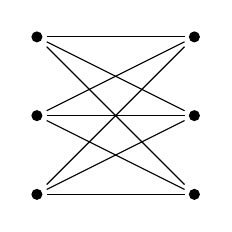
\begin{tikzpicture} % pipartite graph K_{3,3}
      \foreach \i in {1,...,3} {
	\node (n1\i) at (0,\i) {};
	\node (n2\i) at (2,\i) {};
	\fill (n1\i) circle(2pt);
	\fill (n2\i) circle(2pt);
      };
      \foreach \i in {1,...,3}
      {
	\foreach \j in {1,...,3}
	{
	  \path (n1\i) edge (n2\j);
	};
      };
    \end{tikzpicture}
  }
  \caption{Examples for (non-)planar Graphs}
\end{figure}


% triangle (planar)
% square with diagonals (planar) ≅ square with second diagonal non-intersecting
% K_5 (non-planar)
% bipartite graph K_{3,3} (non-planar)

$K_5$ is the smallest non-planar complete graph, $K_{3,3}$ is the smallest non-planar complete bipartite graph.

\begin{definition}
The edges of the graph (which have to be \emph{Jordan curves}) divide the plane into regions. These are the \dt{faces} of the planar graph.
\end{definition}

% Faces of K_4 - Inner: I, II, III, Outer: IV
\begin{figure}[htb] % K4 with the 4 faces labeled
  \centering
  \begin{tikzpicture}
    \fullyConnectedGraph{90,-30,180+30}{2cm}
    \node (n0) at (0,0) {};
    \fill (n0) circle(2pt);
    \foreach \i in {1,...,\the\value{nodecount}} {
      \path (n0) edge (n\i);
    };
    \node at (90+45:0.5cm) {I};
    \node at (45:0.5cm) {II};
    \node at (-90:0.5cm) {III};
    \node at (45:1.5cm) {IV};
  \end{tikzpicture}
  \caption{Faces of $K_4$}
\end{figure}




In the $K_4$, we get
\begin{align*}
    \alpha_0 &= 4 \\
    \alpha_1 &= 6 \\
    \alpha_2 &= 4\quad\text{number of faces}
\end{align*}

\begin{definition}
$H$ is a \dt{subdivision} of $G$ if $H$ is obtained by replacing every edge of $G$ by a path.
\end{definition}
% graph with 4 v and its graph with pathes

\begin{figure}[htb] % K4 and its subdivision
  \centering
  \subfloat[Graph $G$] {
    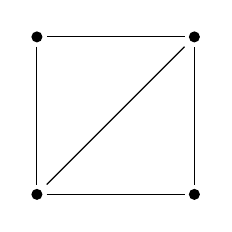
\begin{tikzpicture}
      \node (n1) at (0,0) {};
      \node (n2) at (2,0) {};
      \node (n3) at (2,2) {};
      \node (n4) at (0,2) {};
      \foreach \i in {1,...,4} {
	\fill (n\i) circle(2pt);
      };
      \foreach \i/\j in {1/2, 2/3, 3/4, 4/1, 1/3} {
	\path (n\i) edge (n\j);
      };
    \end{tikzpicture}
  }
  \subfloat[subdivision $H$ of $G$] {
    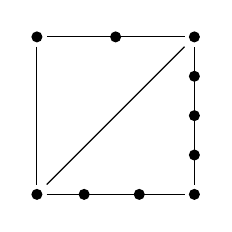
\begin{tikzpicture}
      \node (n1) at (0,0) {};
      \node (n2) at (2,0) {};
      \node (n3) at (2,2) {};
      \node (n4) at (0,2) {};
      \node (n5) at (0.6,0) {};
      \node (n6) at (1.3,0) {};
      \node (n7) at (2,.5) {};
      \node (n8) at (2,1.0) {};
      \node (n9) at (2,1.5) {};
      \node (n10) at (1,2) {};
      \foreach \i in {1,...,10} {
	\fill (n\i) circle(2pt);
      };
      \foreach \i/\j in {1/2, 2/3, 3/4, 4/1, 1/3} {
	\path (n\i) edge (n\j);
      };
    \end{tikzpicture}
  }
  \caption{Graph $G$ and one possible subdivision of $G$ named $H$}
\end{figure}




% Kuratovski's theorem?
\Theorem.
\[
    G\text{ planar} \iff \nexists\;\text{subgraph which is a subdivision of $K_5$ or of $K_{3,3}$.}
\]

\ProofBackward. Trivial if $K_5$ and $K_{3,3}$ non-planar.

\ProofForward. Too hard.

\textbf{Remark (Euler's polyhedron formula).}
\[
    G\text{ connected and planar} \implies
    \underbrace{\alpha_0 - \alpha_1 + \alpha_2}_
        {\text{Euler characteristic}}
    = 2.
\]

% figure of a polyhedron of a dice

\begin{figure}[htb] % polyhedron of a dice
  \centering
    \begin{tikzpicture}
      \drawGraph{1/1, 2/1, 2/2, 1/2, %
                 0/0, 3/0, 3/3, 0/3}%
		{1/2, 2/3, 3/4, 4/1, %
                 5/6, 6/7, 7/8, 8/5, %
	         1/5, 2/6, 3/7, 4/8}
    \end{tikzpicture}
  \caption{Polyhedron of a dice}
\end{figure}





\Proof.
Induction on $\alpha_2$.

Start with $\alpha_2=1$: $G$ is a tree. Then
\[
    \alpha_0-\alpha_1+1 = \alpha_0 - (\alpha_0 + 1) + 1 = 2.
\]

$\alpha_2 = k : k\rightarrow k+1: $
\[
    \text{$G$ has at least $k+1 \geq 2$ faces} \implies
    \exists\;\text{edge separating two faces}
\]
If we remove this edge, we get $G'$.
\begin{align*}
    \alpha_2(G') = k
    \implies &\alpha_0(G') - \alpha_1(G') + \alpha_2(G') = 2
    \implies &\alpha_0(G) - \alpha_1(G) + \alpha_2(G) = 2
\end{align*}

\Lemma.
If $G$ is planar, simple, no cycles of length $3$ (together, this also means no cycles of length $≤ 3$), connected, then
\[
    \alpha_1(G) ≤ 2\alpha_0(G) - 4.
\]

\Proof.
Let $f_j$ be the number of faces with a boundary of length $j$.
Then $f_3 = 0$.
\begin{align*}
\sum_{j≥4} f_j &= \alpha_2 \\
\sum_{j≥4} j f_j &≤ 2\alpha_1
    &&\text{ because each edge is counted at most twice.} \\
4 \sum_{j≥4} f_j ≤ 2\alpha_1
\end{align*}

%\TODO{figure 4 vertices, 3 faces}

\begin{align*}
    \alpha_0 - \alpha_1 + \alpha_2 &≥ 2 \\
    2\alpha_0 - 2\alpha_1 +
    \underbrace{2\alpha_2}_{≤ \alpha_1} &= 4 \\
    4 &≤ 2\alpha_0 - \alpha_1 \\
    \alpha_1 &≤ 2\alpha_0 - 4
\end{align*}

\Remark. In a graph with $k$ components, the Euler characteristic becomes
$\implies \alpha_0 - \alpha_1 + \alpha_2 = 1+k$

\textbf{Corollary.}
$K_{3,3}$ is not planar: Assume it is planar.
$\alpha_0 = 6, \alpha_1 = 9$. As a bipartite graph, it cannot have cycles of length 3: $f_3 = 0$. Therefore, we must have
\[
    \alpha_1 ≤ 2\alpha_0 - 4 \\
    9 ≤ 8
\]
Contradiction! Since $K_{3,3}$ satisfies all other requirements of the lemma, but the inequality does not hold, it cannot be planar.

\begin{definition}
Let $G=(V,E)$ be a planar graph and $F$ the set of faces.
Then $G^* = (V^*, E^*)$ is the \dt{dual} of $G$ with
\begin{align*}
&V^* = F. \\
&F_1F_2 \in E^* &&\text{if their boundaries have a common edge.}
\end{align*}
\end{definition}

% WRONG: \Remark. In general, $G^*$ is a multigraph.
\Remark. $G^*$ is not unique.
% WRONG: \Remark. $\forall v : d(v) ≠ 1 \implies |E| = |E^*|$

%%% corrections from 2013-10-24

\Remark.
\marginpar{corrections \isodate{2013-10-24}}
\begin{compactenum}
  \item $|E| = |E^*|$
  \item In general $|G^*|$ is a multigraph
  \item $G_1, G_2$ are duals of $G \Rightarrow G_1 \cong G_2$
\end{compactenum}

$A \subseteq E$
$A$ cycle in $G \iff A^*$ minimal cut

If G is not necessarily planar: define $G^*$ by (*).
This Graph is unique, if it exists.

\textbf{Theorem (Witness Theorem).} \\
If G is not necessarily planar: define $G^{**}$ by (*)
\begin{compactitem}
  \item $G$ planar $\Rightarrow G^{**} \cong G^*$
  \item $G$ non planar $∄ G^{**}$
\end{compactitem}
% end of last weeks-corrections

\subsection{Bipartite Graphs and Matchings}

\begin{definition}
A simple, undirected graph $G=(V,E)$ is called \dt{bipartite}
iff
\begin{align*}
    V = V_1\cup V_2, V_1\cap V_2 = \varnothing \\
    vw\in E\implies v\in V_1, w\in V_2
\end{align*}
\end{definition}

$K_{n,m}$ is the complete bipartite graph.

\begin{definition}
$M\subseteq E$ is called a \dt{matching} if
\[
    \forall e,f\in M: e,f\text{ have no vertex in common.}
\]
\end{definition}
\begin{definition}
In a \dt{perfect matching},
\[
    \forall v\in V: v\text{ incident to some }e\in M.
\]
\end{definition}

\begin{figure}[htb] % perfect matching
  \centering
    \begin{tikzpicture}
      \drawGraph{0/0, 0/1, 0/2, 1/0, 1/1, 1/2}%
                {1/2, 2/3, 1/6, 1/4, 3/5, 4/5, 5/6}
      \foreach \i/\j in {1/5, 2/4, 3/6} {
	\draw[red, very thick] (n\i) -- (n\j);
      };
    \end{tikzpicture}
  \caption{Graph with perfect matching in red}
\end{figure}



